\subsection{UC1 - Creazione ambiente}
\label{sub:uc1}

%TODO: Add correct image
% Se uno use case esce dalla post allora non mettiamo in scenario secondario ma in estensione
% se invece la post rimane la stessa non è estensione.

\begin{figure}[h]
    \centering
    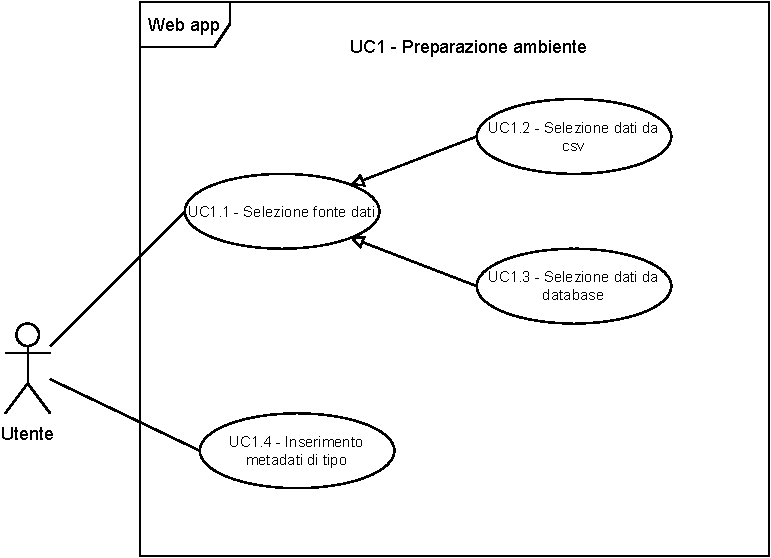
\includegraphics[width=0.7\textwidth]{diagrammi/UC1.pdf}
    \caption{Diagramma rappresentante UC1}
    \label{fig:UC1}
\end{figure}


\begin{itemize}
    \item \textbf{Descrizione}: L'utente prepara l'applicativo HD Viz alla visualizzazione dei dati importando un opportuno dataset e assegna, se non già definiti, dei metadati che descrivono il tipo del dato di ogni sua dimensione.
	
    \item \textbf{Attore primario}: Utente;
    \item \textbf{Attore secondario}: Database;
    
    
    \item \textbf{Precondizione}:   L'utente decide di caricare i dati;

    \item \textbf{Postcondizione}:  Viene caricato un dataset e ogni sua dimensione del ha associato
                                    dei metadati;

	\item \textbf{Scenario principale}:
		\begin{enumerate}
			\item L'utente seleziona l'opzione di aggiunta dei dati;
            \item L'utente seleziona la fonte dei dati da importare e li importa;
            \item Il dataset caricato è corretto e provvisto di metadati validi.
        \end{enumerate}
   
    \item \textbf{Scenari alternativi}:
		\begin{itemize}
            \item Il dataset caricato presenta metadati di tipo non validi o ne è sprovvisto:
            \begin{enumerate}
                \item L'utente inserisce manualmente i metadati di tipo mancanti (\hyperref[ssub:uc1.4]{UC1.4}).
            \end{enumerate}
        \end{itemize}
\end{itemize}

\subsubsection{UC1.1 - Inserimento dati}
\label{ssub:uc1.1}
\begin{itemize}
    \item \textbf{Descrizione}: L'utente decide di impostare l'ambiente creando un dataset i cui 
                                dati vengono caricati da file csv oppure da database al quale l'utente ha accesso;

    \item \textbf{Attore primario}: Utente;
    \item \textbf{Attore secondario}: Database;
    
    \item \textbf{Precondizione}:   L'utente decide di caricare i dati;

    \item \textbf{Postcondizione}:  Viene caricato un dataset non vuoto dalla fonte scelta dall'utente;

	\item \textbf{Scenario principale}:
		\begin{enumerate}
			\item L'utente seleziona l'opzione di aggiunta dei dati:
            \item Viene caricato un dataset dalla fonte scelta dall'utente.
        \end{enumerate}

        \item \textbf{Generalizzazioni}:
        \begin{enumerate}
            \item Inserimento dati da file csv (\hyperref[ssub:uc1.2]{UC1.2};
            \item Inserimento dati da database (\hyperref[ssub:uc1.3]{UC1.3}).
        \end{enumerate}
\end{itemize}


\subsubsection{UC1.2 - Inserimento dati da file csv}
\label{ssub:uc1.2}
\begin{itemize}
    \item \textbf{Descrizione}: L'utente importa un dataset non vuoto da un file csv del suo dispositivo;

    \item \textbf{Attore primario}: Utente;
    
    \item \textbf{Precondizione}:   L'utente selezione l'opzione di caricare i dati da un file csv;
    \item \textbf{Postcondizione}:  Viene caricato un dataset;

	\item \textbf{Scenario principale}:
		\begin{enumerate}
			\item L'utente seleziona l'opzione di aggiunta dei dati mediante file;
			\item L'utente seleziona il file csv di dati valido da importare.
        \end{enumerate}

    \item \textbf{Estensioni}:
    \begin{itemize}
        \item Se il caricamento da file fallisce:
        \begin{enumerate}
            \item Il caricamento del dataset viene interrotto;
            \item Viene visualizzato un messaggio di errore (\hyperref[sub:uc6]{UC6}).
        \end{enumerate}
    \end{itemize}
\end{itemize}

\newpage
\begin{figure}[h]
    \centering
    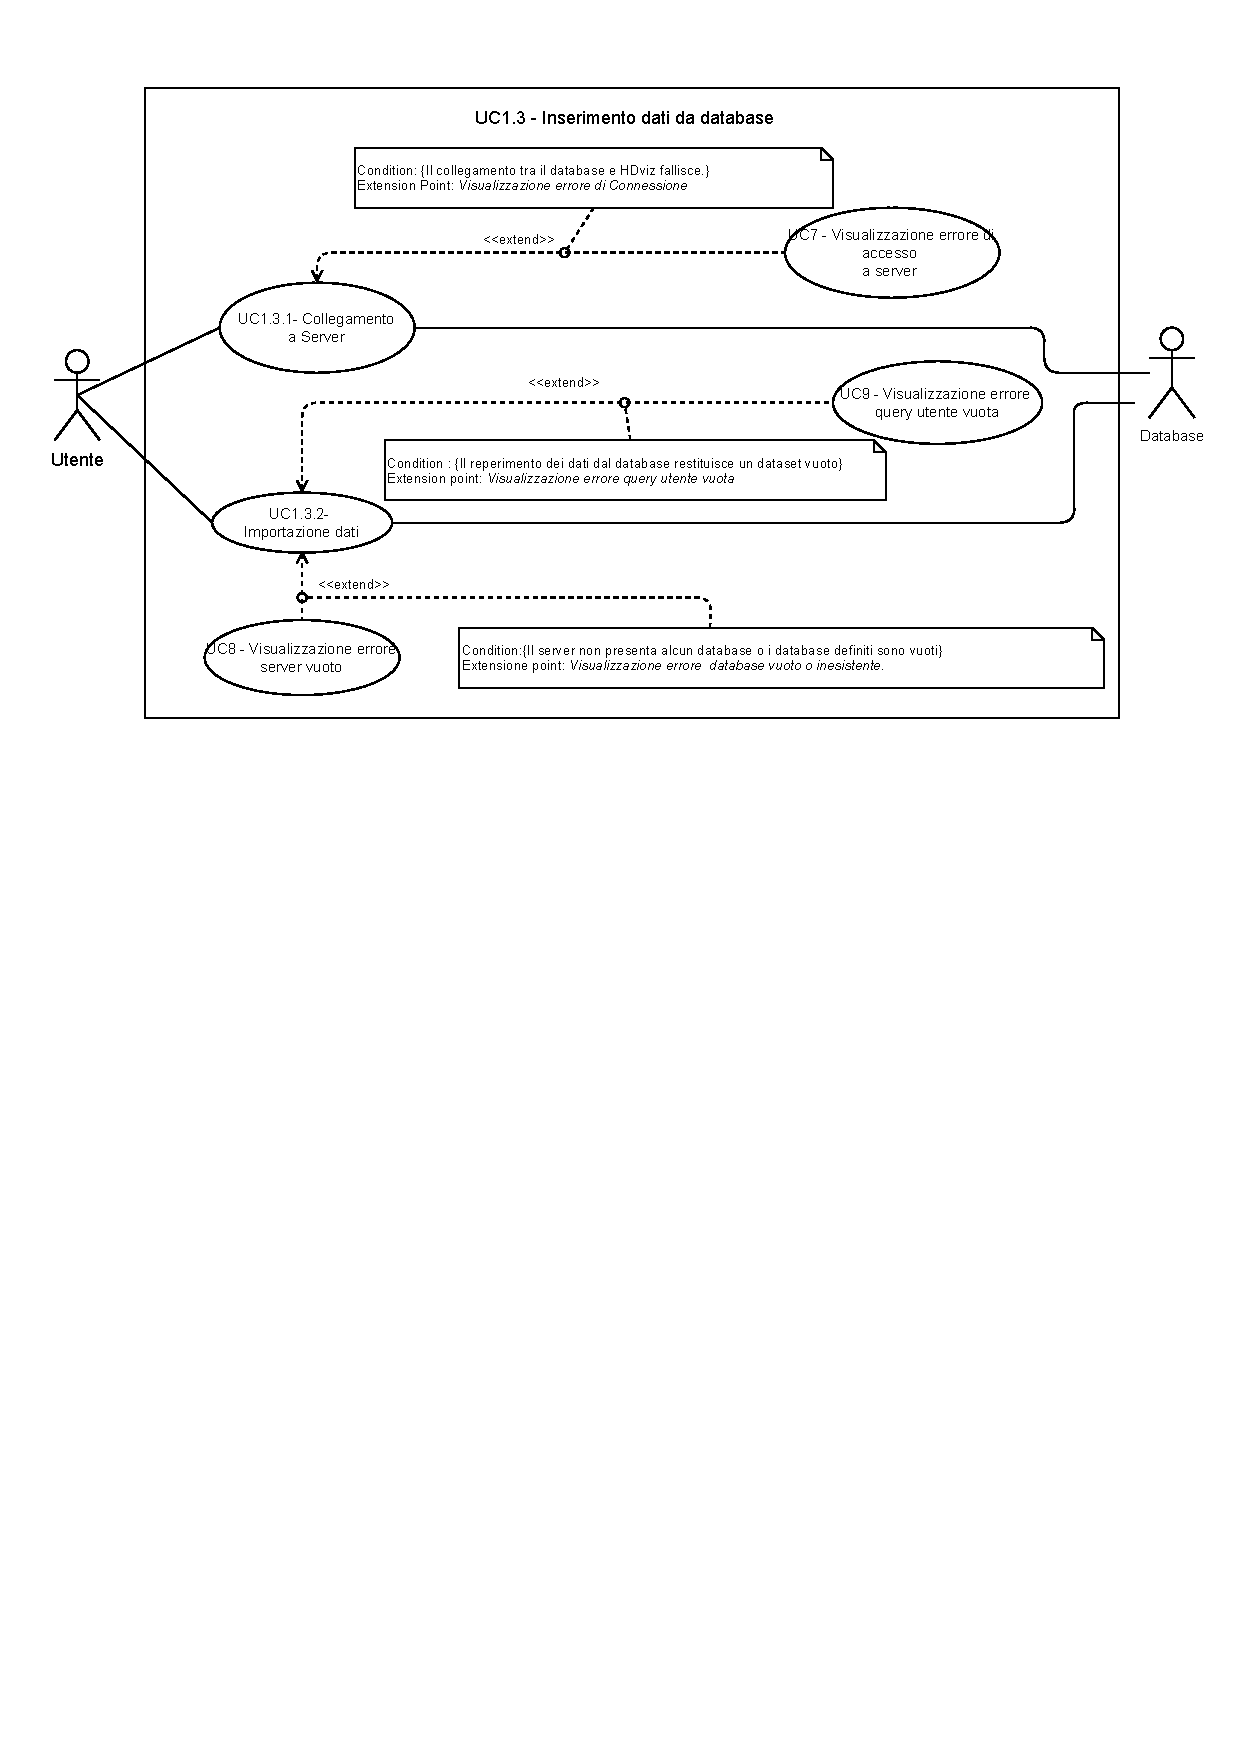
\includegraphics[width=0.9\textwidth]{diagrammi/UC1_3.pdf}
    \caption{Diagramma rappresentante UC1.3}
    \label{fig:UC1.3}
\end{figure}


\subsubsection{UC1.3 - Inserimento dati da database}
\label{ssub:uc1.3}
\begin{itemize}
    \item \textbf{Descrizione}: L'utente si connette ad un database di cui dispone accesso e 
                                crea un dataset non vuoto dal risultato di una ricerca delle tabelle che gli interessano
                                visualizzare successivamente in HD Viz;
    \item \textbf{Attore primario}: Utente;
    
    \item \textbf{Attore secondario}: Database;
    
    \item \textbf{Precondizione}:   L'utente decide di caricare i dati mediante un database;
    \item \textbf{Postcondizione}:  Viene caricato un dataset da un database; 

	\item \textbf{Scenario principale}:
		\begin{enumerate}
			\item L'utente effettua la connessione con un database da lui fornito (\hyperref[par:uc1.3.1]{UC1.3.1});
			\item L'utente importa i dati dal form di caricamento dati (\hyperref[par:uc1.3.2]{UC1.3.2}).
        \end{enumerate}

    \item \textbf{Estensioni}:
    \begin{itemize}
        \item Se l'apertura della connessione con il database fallisce:
        \begin{enumerate}
            \item L'inserimento dei dati viene interrotto;
            \item Viene visualizzato un messaggio di errore (\hyperref[sub:uc7]{UC7}).
        \end{enumerate}

        \item Se il server al quale si è connessi non ha database o tutti sono vuoti:
        \begin{enumerate}
            \item L'inserimento dei dati viene interrotto;
            \item Viene visualizzato un messaggio di errore (\hyperref[sub:uc8]{UC8}).
        \end{enumerate}

        \item Se la query utente è vuota:
        \begin{enumerate}
            \item L'inserimento dei dati viene interrotto;
            \item Viene visualizzato un messaggio di errore (\hyperref[sub:uc9]{UC9}).
        \end{enumerate}
    \end{itemize}
\end{itemize}


\newpage
\begin{figure}[h]
    \centering
    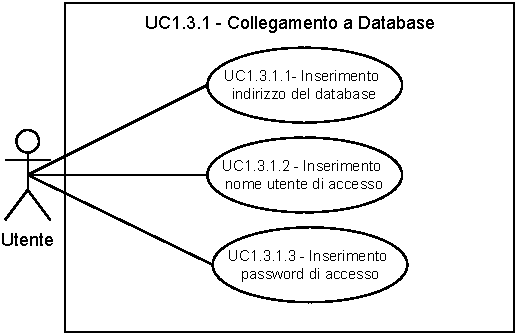
\includegraphics[width=0.5\textwidth]{diagrammi/UC1_3_1.pdf}
    \caption{Diagramma rappresentante UC1.3.1}
    \label{fig:UC1.3.1}
\end{figure}


\paragraph{UC1.3.1 - Collegamento a Server}
\label{par:uc1.3.1}
\begin{itemize}
    \item \textbf{Descrizione}: L'utente apre una connessione con un server di dati del quale 
                                dispone le credenziali di accesso;

    \item \textbf{Attore primario}: Utente;
    \item \textbf{Attore secondario}: Database;
    
    \item \textbf{Precondizione}:   L'utente decide di caricare i dati mediante un database;
    \item \textbf{Postcondizione}:  Viene aperta la connessione con un server di dati;

	\item \textbf{Scenario principale}:
		\begin{enumerate}
			\item L'utente immette i campi necessari per l'acceso: indirizzo, nome utente e password;
			\item HD Viz si connette al server con i valori immessi dall'utente.
        \end{enumerate}
    \end{itemize}


\subparagraph{UC1.3.1.1 - Inserimento indirizzo}
\label{spar:uc1.3.1.1}
\begin{itemize}
    \item \textbf{Descrizione}: L'utente inserisce l'indirizzo del server al quale vuole accedere;
    \item \textbf{Attore primario}: Utente;
   
    \item \textbf{Precondizione}:   L'utente decide di caricare un dataset mediante un database;
    \item \textbf{Postcondizione}:  Viene inserito l'indirizzo del server di dati;
    
    \item \textbf{Scenario Principale}: 
    \begin{enumerate}
        \item L'utente inserisce l'indirizzo di connessione.
    \end{enumerate}

\end{itemize}


\subparagraph{UC1.3.1.2 - Inserimento nome utente}
\label{spar:uc1.3.1.2}
\begin{itemize}
    \item \textbf{Descrizione}: L'utente inserisce il nome utente per accedere al server;
    \item \textbf{Attore primario}: Utente;
    
    \item \textbf{Precondizione}:   L'utente decide di caricare i dataset mediante un database;
    \item \textbf{Postcondizione}:  Viene inserito il nome utente per l'accesso al server di dati;

    \item \textbf{Scenario Principale}: L'utente inserisce il nome d'accesso.
\end{itemize}


\subparagraph{UC1.3.1.3 - Inserimento password}
\label{spar:uc1.3.1.3}
\begin{itemize}
    \item \textbf{Descrizione}: L'utente inserisce la password per accedere al server;
    \item \textbf{Attore primario}: Utente;
    
    \item \textbf{Precondizione}:   L'utente decide di caricare i dataset mediante un database;
    \item \textbf{Postcondizione}:  Viene caricato un dataset dal database;

    \item \textbf{Scenario Principale}: L'utente inserisce la password d'accesso.

\end{itemize}

%TODO: Inserimento anche di database (non fa formalmente parte di una query)
\paragraph{UC1.3.2 - Importazione dati}
\label{par:uc1.3.2}
\begin{itemize}
    \item \textbf{Descrizione}: L'utente ottiene i dati che da inserire nel nuovo dataset da un database
                                del server con cui ha una connessione aperta al momento, mediante 
                                l'esecuzione di una query personalizzata che fornisce in un form;

    \item \textbf{Attore primario}: Utente;
    
    \item \textbf{Attore secondario}: Database;
    
    \item \textbf{Precondizione}:   L'utente ha aperto una connessione con un server dati;
    \item \textbf{Postcondizione}:  Viene costruito il dataset dai dati reperiti dall'utente mediante un file di query;

	\item \textbf{Scenario principale}:
        \begin{enumerate}
            \item L'utente seleziona il database del server sul quale fare la selezione;
			\item L'utente inserisce nel form una query per il riperimento dei dati che viene eseguita sul server;
			\item Viene costruito il dataset dal risultato della ricerca.
        \end{enumerate}
    %TODO Capire dove diamine vanno messe le estensioni.
\end{itemize}

\subsubsection{UC1.4 - Inserimento metadati}
\label{ssub:uc1.4}
\begin{itemize}
    \item \textbf{Descrizione}: L'utente assegna ad ogni dimensione del dataset importato, in cui non fossero già 
    correttamente definiti, i relativi metadati che descrivono il tipo di dato;

    \item \textbf{Attore primario}: Utente;
    
    \item \textbf{Precondizione}:   L'utente ha caricato un dataset e non tutti i suoi metadati sono validi o definiti;
    \item \textbf{Postcondizione}:  Il dataset caricato è provvisto di metadati validi;

	\item \textbf{Scenario principale}:
		\begin{enumerate}
            \item L'utente assegna ad ogni dimensione del dataset il relativo metadato di tipo scegliendo tra:
                    Nominale, Ordinale, Intervallo o Rapporto.
        \end{enumerate}

\end{itemize}

